For the users with a local installation of OpenQuake, the input files 
for this demostration can be found in the folder 
\texttt{/media/vbox/ssa\_demo}.
\marginpar{What about OATS users?}
%
% -----------------------------------------------------------------------------
\section{Model description}
%
The model used for this exercise corresponds to the one proposed by 
\citet{midzi1999} in the context of the GSHAP project.
As illustrated in Figure \ref{fig:ssa_area_sources}, it contains 21 
area sources distributed along a wide band ideally connecting the 
Red Sea with South Africa.

The area sources part of this model can be ideally subdivided into a small 
number of groups.
%
To the north, a first set of area sources covers the three branches 
of the triple junction in the Afar region. 
The following set shows a spatial pattern reproducing the structural 
trend of the graben systems composing the two main branches composing 
the continental part of the East African Rift: the Western and East 
branches. 
The last set of sources includes the southermost part of the model 
where Rift's textonic structure are less evident and the seismicity 
spreads over a wide sectors (see Figure \ref{fig:Subsahara_Catalogue_ISC_1}).
%
\begin{figure}[!ht]
	\centering
	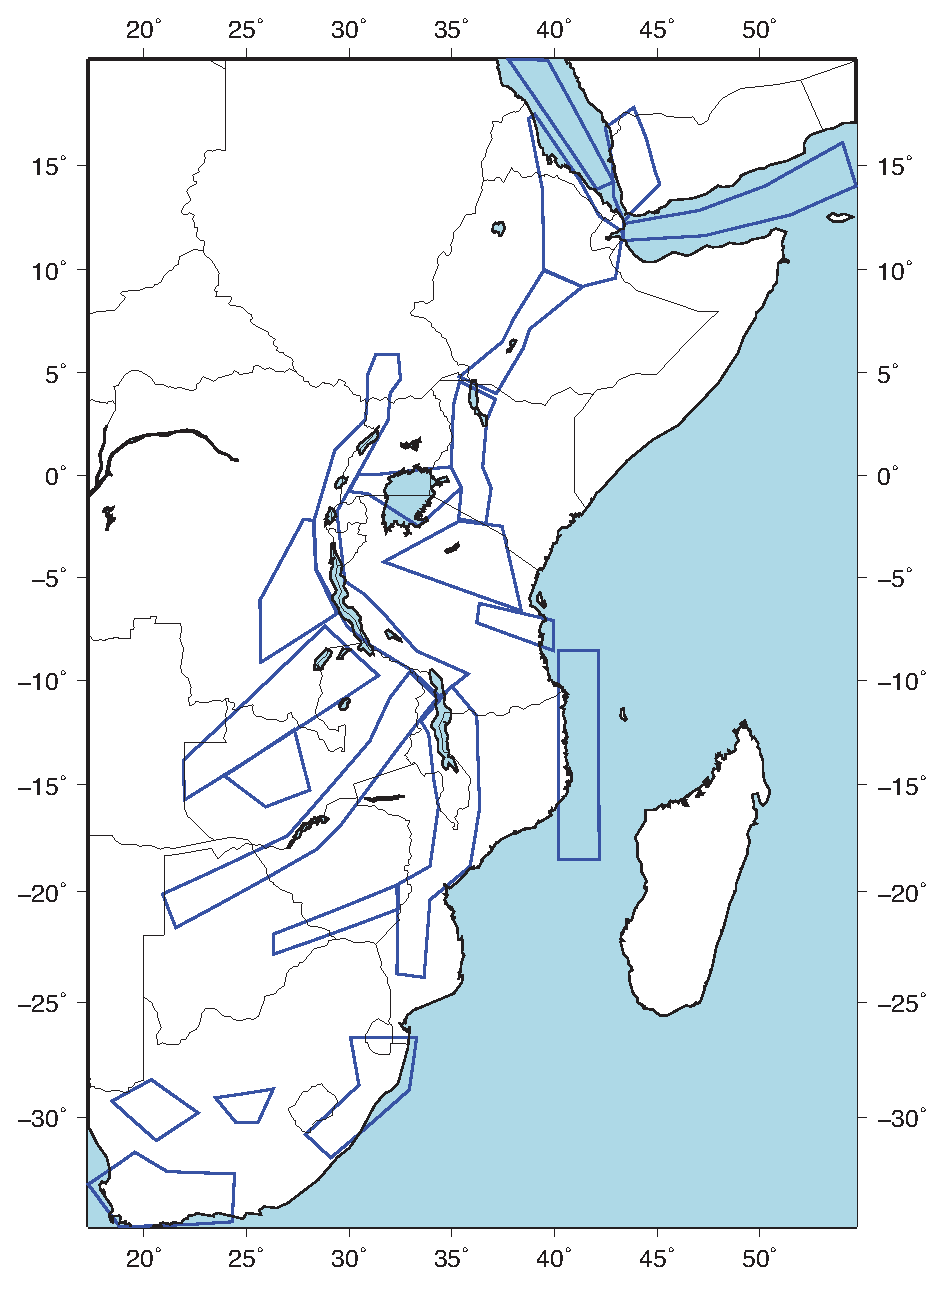
\includegraphics[width=14cm]
        {./figures/ssa_area_sources.eps}
	\caption{Area sources in the demo PSHA input model.}
	\label{fig:ssa_area_sources}
\end{figure}
%
The seismicity recurrence parameters and the maximum magnitude 
assigned to the different sources corresponds to the ones originally
determined by \citet{midzi1999}.

The maximum magnitude of the seismic sources ranges between 6.5 
and 7.8; the sources with the highest potential are zone 6 and 7.  
Areas 4 and 6 are the ones with the highest occurrence rates.
%
% -----------------------------------------------------------------------------
\section{Assignment: hazard calculation using the demonstration model}
%
The first proposed assignment aims at computing hazard for a small area 
along the rift valley using Openquake and the PSHA input model 
provided.

The exercise will consist on:
\begin{itemize}
    \item computing hazard curves for some (at least 4) of the cities 
        in the eastern part of Sub-Saharan Africa (see Table \ref{tab:cities})
        \begin{table}
            \centering
            \begin{tabular}{llrr} \hline
            \bf{Nation} & \bf{City} & \bf{Lon} & \bf{Lat} \\ \hline
            Botswana    & Gaborone  & 25.92 & -24.65 \\
            Burundi     & Bujumbura & 29.37 &  -15.36 \\
            Ethiopia    & Addis Ababa & 38.75 &  9.04 \\
            Kenia       & Nairobi   & 36.73 &  -1.28 \\
            Malawi      & Lilingwe  & 28.37 &  -13.96 \\
            Mozambique  & Maputo    & 32.61 & -25.93 \\
            Rwanda      & Kigali    & 28.37 &  -1.95 \\
            South Africa & Cape Town & & \\
            Tanzania    & Dodoma    & 35.75 &  -6.16 \\
            Uganda      & Kampala   & 32.61 &  0.28 \\
            Zambia      & Lusaka    & 28.29 &  -15.43 \\
            Zimbawe     & Harare    & 31.12 &  -17.85 \\
            \hline
            \end{tabular}
            \label{tab:cities}
            \caption{List of cities to be used in the first part of exercise}
        \end{table}
    \item computing a hazard map for a small area with opposite vertexes 
        correponding to: 
        \begin{itemize}
            \item Lower left (lon: 30.0 lat: -10.0)
            \item Upper right (lon: 35.0 lat: -5.0)
        \end{itemize}
    \item disaggregate the PGA with 10\% probability of exceedance in 50 
        years in XXX
\end{itemize}
%
For each of the proposed exercises it is important to create (or modify) 
the configuration file particularly for what conserns the investigated 
area (or sites) and the type of analysis to be completed.
